\documentclass{beamer}
\usepackage{animate}
\usepackage{ulem}
\usepackage{multicol}
\usepackage{multimedia}
\usepackage{graphicx}
\usepackage{caption}
\usepackage{subcaption}
\usepackage{hyperref}
\usepackage{verbatim}
\usepackage{amsmath}
\usepackage[latin1]{inputenc}
\usetheme{fel}
\usepackage[scaled=0.6]{helvet}

\title[Hermes library]{Hermes library \\ Rapid hp-FEM \& hp-DG Solver Toolkit}
\author[hp-FEM group]{Lukas Korous et al.}
\institute[Pilsen, Reno]{hp-FEM group, University of Nevada, Reno; University of West Bohemia, Pilsen\\ }

\begin{document}

\begin{frame}
\titlepage
\end{frame}


\begin{frame}
\begin{enumerate}
\item When Hermes comes in handy
\item Easy installation description (Linux / Windows)
\item Learning resources availability
\item Code customizations / extensions
\item Features show off
\end{enumerate}
\end{frame}

\newcommand{\bb}[1]{\textbf{\Large{#1}}}
\newcommand{\bbb}[1]{\textbf{\Large{\textcolor[rgb]{0,0.29,0.75}{#1}}}}

\section{When Hermes comes in handy}
\begin{frame}
	\begin{itemize}
		\item \Large{Algorithms testing, methods comparison}
			\begin{itemize}
				\item \small
				D. Pugal, P. Solin, J. K. Kim, A. Aabloo: Modeling Ionic Polymer-Metal Composites with Space-Time Adaptive Multimesh hp-FEM, Communications in Computational Physics 2012, 11 (249-270) 
				\item \small
				M. Bittl, D.Kuzmin: An hp-adaptive flux-corrected transport algorithm for continuous finite elements, Computing, May 2013, 95-1 Supplement (27-48)
			\end{itemize}
		\item \Large{Adaptive algorithms benchmarking}
			\begin{itemize}
				\item \small
				P. Solin, O. Certik, L.Korous: Three anisotropic benchmark problems for adaptive finite element methods, Applied Mathematics and Computation, 2013, 219-13 (7286-7295)
				\item \small
				Z. Ma, L. Korous, E. Santiago: Solving a suite of NIST benchmark problems for adaptive FEM with the Hermes library, Journal of Computational and Applied Mathematics, 2012, 236-18 (4846-4861)
			\end{itemize}
		\item \Large{Easy solver prototyping}
		  \vspace{-3mm}
		  \begin{multicols}{2}
			\begin{itemize}
				\item \small Acoustics, Wave propagation
				\item \small  Compressible \& Incompressible Flow
				\item \small  Flame Propagation
				\item \small  Maxwell'ss equations (transient, harmonic)
				\item \small  Linear Elasticity, Thermoelasticity
				\item \small  Gross-Pitaevski, Nernst-Planck
				\item \small  Neutronics (Milan Hanus - NTIS, UWB)
				\item \small  Richards Equation
				\item \small  ...
			\end{itemize}
			\end{multicols}
	\end{itemize}
\end{frame}

\section{When Hermes comes in handy}
\begin{frame}
	\begin{itemize}
		\item \small  Acoustics, Wave propagation \hspace{15mm} 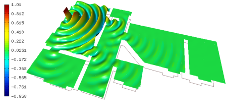
\includegraphics[height=.06\textheight]{outputs/apartment-sol.png} 
		\item \small  Compressible \& Incompressible Flow \hspace{36mm}  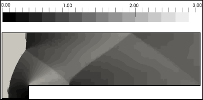
\includegraphics[height=.06\textheight]{outputs/sln4.png} 
		\item \small  Flame Propagation \hspace{25mm}  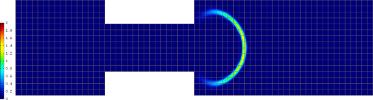
\includegraphics[height=.06\textheight]{outputs/sol31.png} 
		\item \small  Maxwell'ss equations (transient, harmonic) \hspace{31mm}  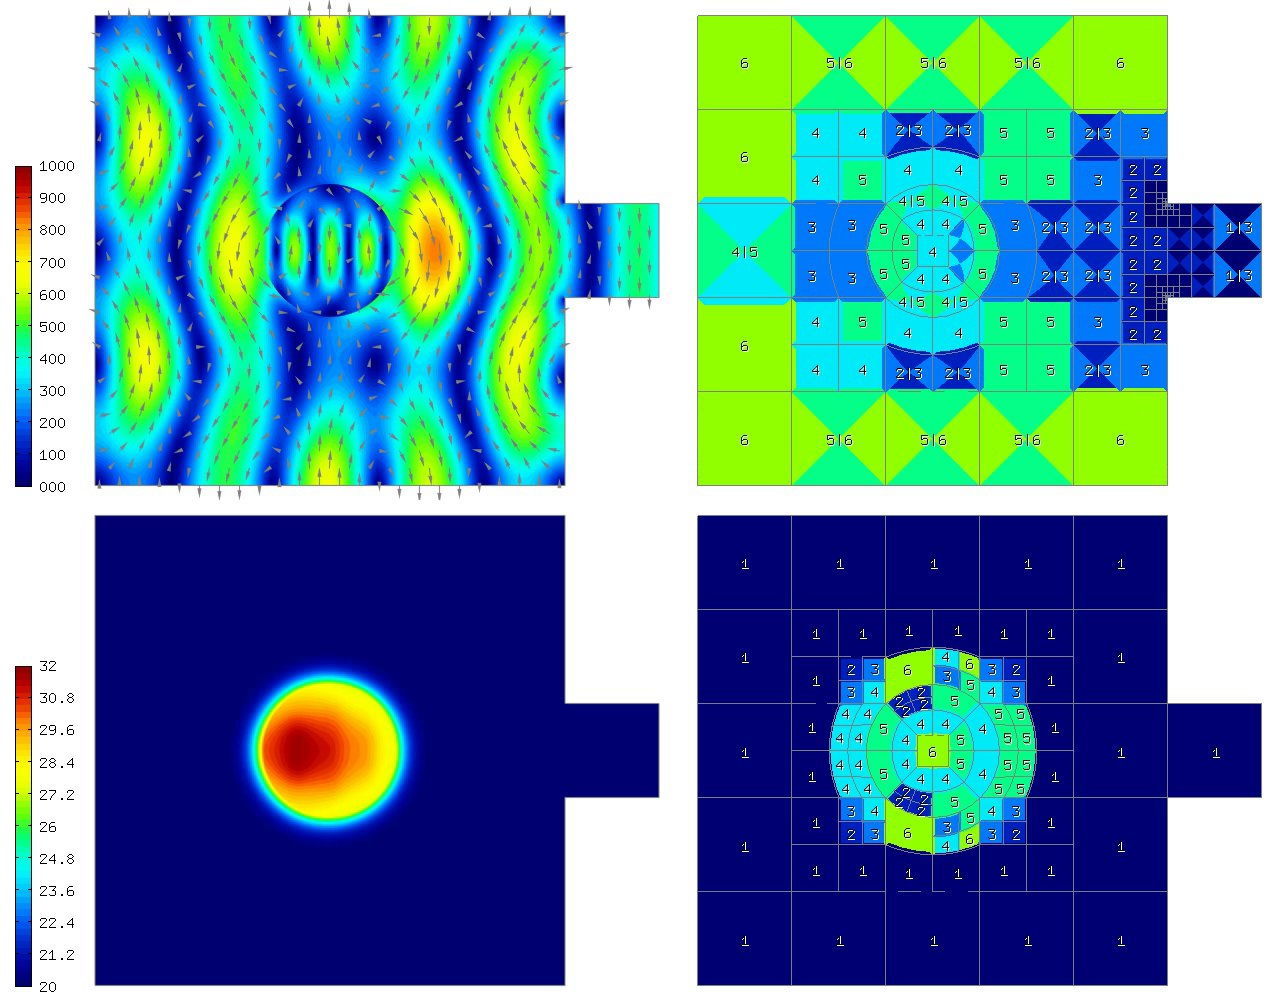
\includegraphics[height=.06\textheight]{outputs/micro.jpg} 
		\item \small  Linear Elasticity, Thermoelasticity \hspace{12mm}  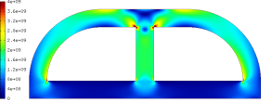
\includegraphics[height=.06\textheight]{outputs/mises.png} 
		\item \small  Gross-Pitaevski  \hspace{56mm} 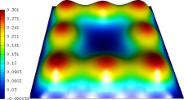
\includegraphics[height=.06\textheight]{outputs/sol_2.png} 
		\item \small  Neutronics (Milan Hanus - NTIS, UWB) \hspace{6mm}  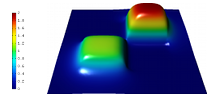
\includegraphics[height=.06\textheight]{outputs/neutro_1.png} 
		\item \small  Richards Equation  \hspace{53mm} 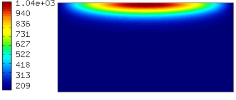
\includegraphics[height=.06\textheight]{outputs/rich.png}
	\end{itemize}
\end{frame}

\section{Easy installation}
\begin{frame}
Industry standard tools
\begin{itemize}
\item \bb{Git}, github.com
\item \bb{CMake} multiplatform build system
\item Code compliant with \bb{g++}, \bb{MSVC} 2010 and newer
\item \bb{Doxygen} documentation available online
\item \bb{XML} exportable \& importable entities
\item \bb{OpenGL} visualization \& VTK, Tecplot outputs
\item No Fortran - only \bb{C++}
\end{itemize}
\end{frame}

\subsection{Linux}
\begin{frame}
Primary supported distribution is Ubuntu, Debian. The following is the complete procedure how to install Hermes\ \\ \ \\
	\begin{enumerate}
		\item sudo apt-get install git git-core cmake g++ freeglut3-dev libsuitesparse-dev libglew-dev libxerces-c-dev xsdcxx
		\item git clone git@github.com:hpfem/hermes.git
		\item cd hermes
		\item cmake .
		\item make -j\#
		\item sudo make install
	\end{enumerate}
\end{frame}

\subsection{Windows}
\begin{frame}
Microsoft Visual Studio is the primary supported compiler, IDE and debugger on Windows. The following is the complete procedure how to build Hermes\ \\ \ \\
	\begin{enumerate}
		\item Download prerequisities from http://www.hpfem.org/hermes/building-and-using-hermes-on-windows/
		\item Download Git client (git-scm.com/) and CMake (cmake.org/)
		\item git clone git@github.com:hpfem/hermes.git
		\item cd hermes
		\item cmake -G Visual Studio \#
		\item devenv.exe hermes.sln
		\item Build
	\end{enumerate}
\end{frame}

\section{Learning resources}
\begin{frame}
	\begin{itemize}
		\item \bbb{Library documentation}
			\begin{itemize}
				\item \bb{HTML} - http://hpfem.org/hermes-doc/hermes/html/index.html
				\item \bb{PDF} - http://hpfem.org/hermes-doc/hermes/hermes.pdf
			\end{itemize}
		\item \bbb{Tutorial \& Examples}
			\begin{itemize}
				\item \bb{Tutorial} - http://hpfem.org/hermes-doc/hermes-tutorial/html/index.html
				\item \bb{Examples} - http://hpfem.org/hermes-doc/hermes-examples/html/index.html
			\end{itemize}
		\item \bbb{Doxygen documentation}
			\begin{itemize}
				\item \bb{Common} (dimension independent) tools: http://hpfem.org/hermes-doc/hermes/hermes\_common/index.php
				\item \bb{Hermes2D} http://hpfem.org/hermes-doc/hermes/hermes2d/index.php
			\end{itemize}
	\end{itemize}
\end{frame}


\section{Coding with Hermes}
\subsection{Mesh}
\begin{frame}
	\begin{figure}[H]
		\centering

		\begin{subfigure}{0.4\textwidth}
			\vspace{-20mm}
			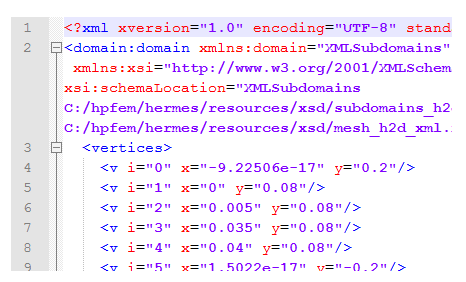
\includegraphics[width=.95\textwidth]{codeimg/meshFile.png}
			\caption{XML mesh format}
		\end{subfigure}
		\begin{subfigure}{0.55\textwidth}
			\hspace{20mm}
			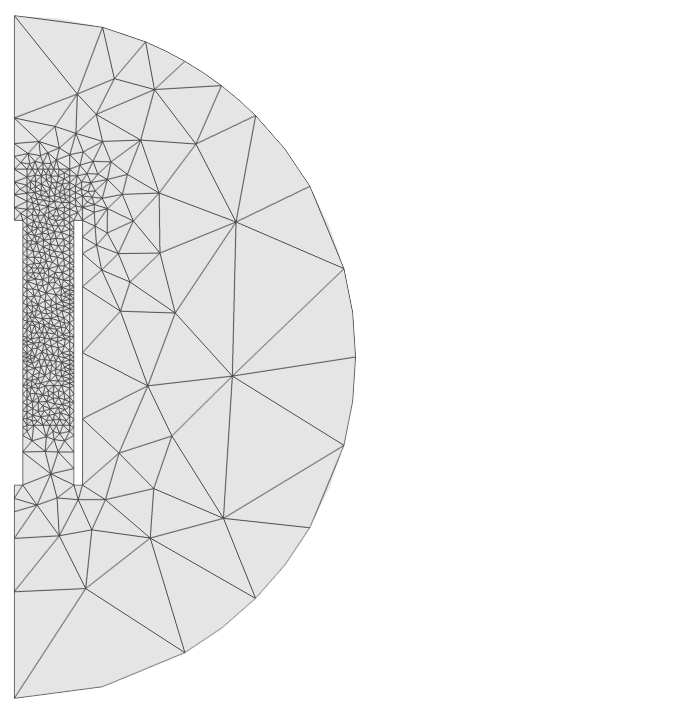
\includegraphics[width=.95\textwidth]{screenshots/mesh.png}
			\caption{Mesh visualized using OpenGL}
		\end{subfigure}
		\ \\
		\vspace{-25mm}
		\hspace{-60mm}
		\begin{subfigure}{0.4\textwidth}
			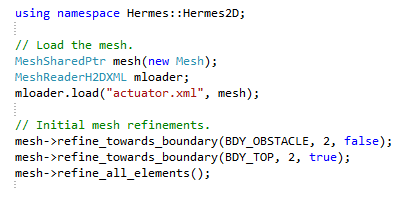
\includegraphics[width=.95\textwidth]{codeimg/meshCode.png}
			\caption{Hermes2D classes to handle mesh}
		\end{subfigure}
	\end{figure}
	\end{frame}


\subsection{Space, boundary conditions}
\begin{frame}
	\begin{figure}[H]
		\centering
		\begin{subfigure}{0.9\textwidth}
			\centering
			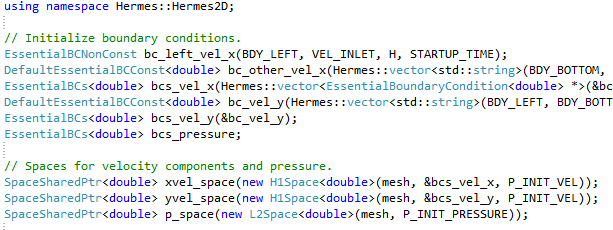
\includegraphics[width=.69\textwidth]{codeimg/spaceBcs.png}
			\vspace{-3mm}
			\caption{BCs and Space handling in Hermes2D}
		\end{subfigure}
		\ \\
		\begin{subfigure}{.47\textwidth}
		\centering
			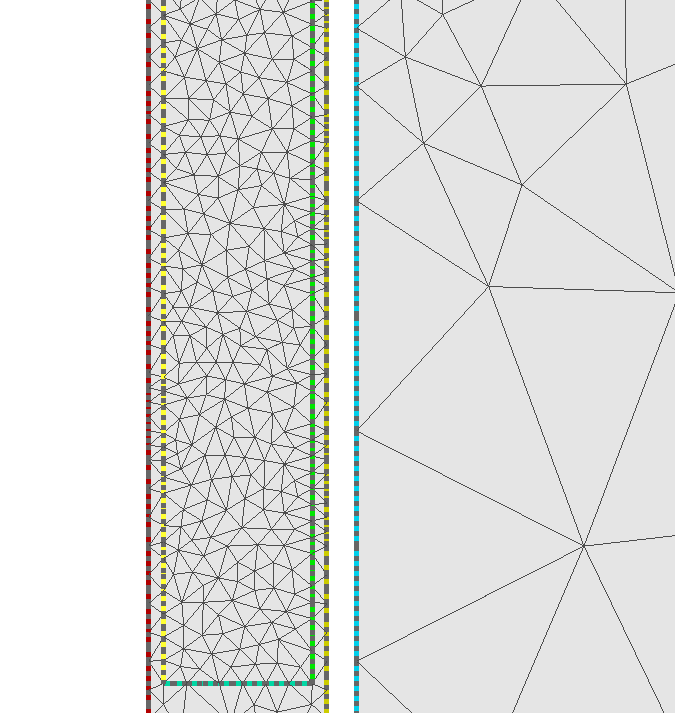
\includegraphics[width=.6\textwidth]{screenshots/bcs.png}
			\caption{Boundary markers}
		\end{subfigure}
		\begin{subfigure}{.47\textwidth}
		\centering
			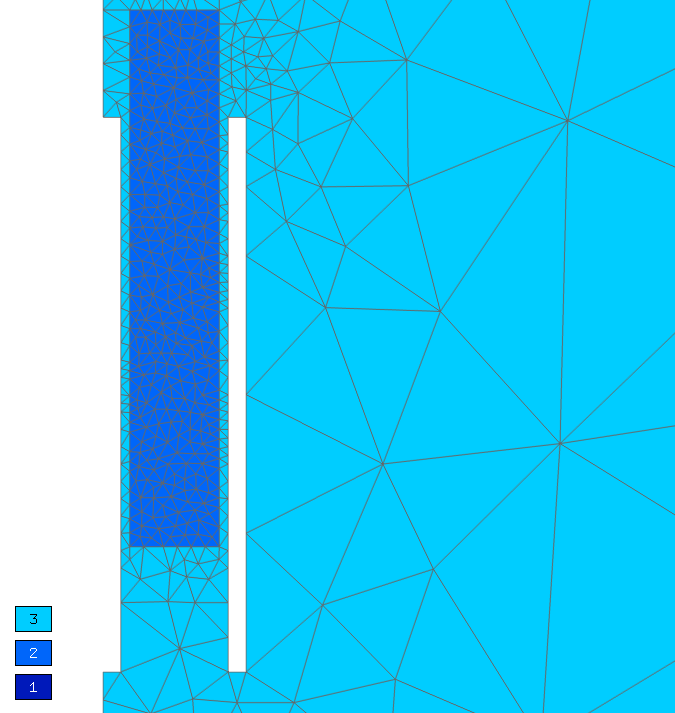
\includegraphics[width=.6\textwidth]{screenshots/space.png}
			\caption{Space - polynomial order}
		\end{subfigure}
	\end{figure}
\end{frame}


\subsection{Weak formulation}
\begin{frame}
\begin{figure}[H]
		\centering
		\begin{subfigure}{0.9\textwidth}
			\centering
			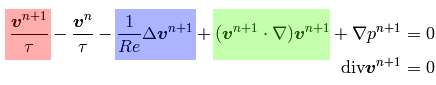
\includegraphics[width=.65\textwidth]{codeimg/NSEquations.png}
			\vspace{-3mm}
			\caption{Navier-Stokes equations (strong formulation)}
		\end{subfigure}
		\ \\
		\vspace{13mm}
		\begin{subfigure}{.95\textwidth}
		\centering
			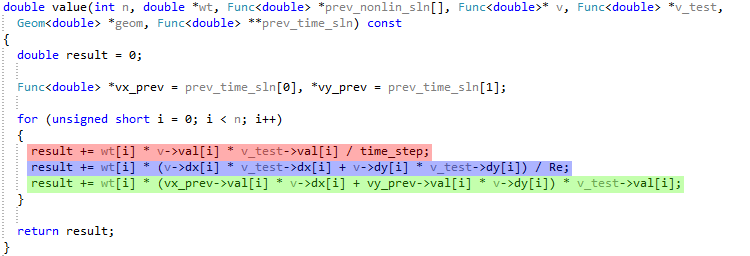
\includegraphics[width=.94\textwidth]{codeimg/weakForm.png}
			\vspace{-5mm}
			\caption{Weak formulation in Hermes2D}
		\end{subfigure}
	\end{figure}
\end{frame}


\subsection{Solvers - linear and nonlinear (and others)}
\begin{frame}
\begin{minipage}{.49\textwidth}
Linear ones are easy:\ \\
\vspace{10mm}
\begin{figure}
	\centering
	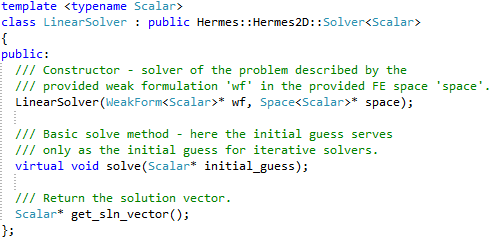
\includegraphics[width=.9\textwidth]{codeimg/linearSolver.png}
	\vspace{-4mm}
	\caption{Linear solver API}
\end{figure}
\vspace{20mm}
\end{minipage}
\begin{minipage}{.49\textwidth}
For nonlinear ones we need more weaponry:
\begin{figure}
	\centering
	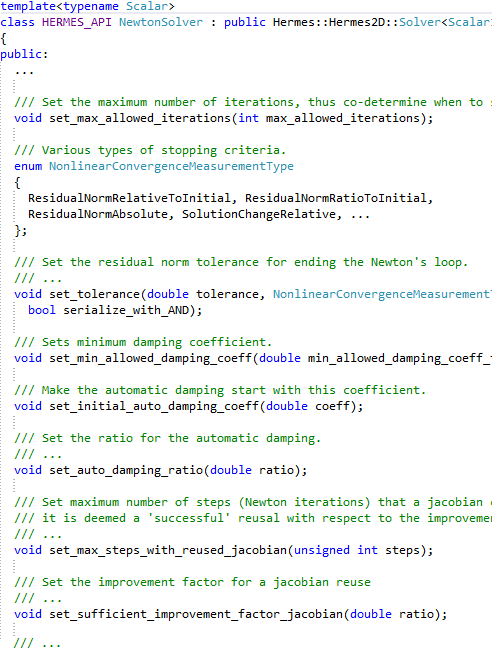
\includegraphics[width=.9\textwidth]{codeimg/nonlinearSolver.png}
	\vspace{-4mm}
	\caption{Newton solver API}
\end{figure}
\end{minipage}

\end{frame}


\subsection{Adaptivity}
\begin{frame}
\begin{itemize}
\item Hermes can do hp-adaptivity with or without a reference solution.
\item The reference solution approach is probably the most general.
\item A common sense implementation would
\begin{enumerate}
\item create a reference space from the currently considered (coarse) space
\item solve (using e.g. NewtonSolver) the problem in the fine space
\item solve in the coarse space
\item subtract \& express the difference as a function (is this trivial and cheap?)
\item use the difference as data to decide whether to split in $h$ or in $p$ (how?)
\item refine the space as decided and continue from top (is this trivial and cheap?)
\end{enumerate}
\end{itemize}
\end{frame}

\begin{frame}
\begin{itemize}
\item Our implementation does more or less the same thing
\begin{enumerate}
\item create a reference space from the currently considered (coarse) space
\item solve (using e.g. NewtonSolver) the problem in the fine space
\item \sout{solve in the coarse space} Perform an orthogonal projection of the solution from the fine to the coarse space (much cheaper).
\item subtract \& express the difference as a function (Is this trivial and cheap? \textcolor[rgb]{1,0,0}{Somehow.})
\begin{itemize}
\item Because we have both the coarse and fine component in hand, we can calculate the difference locally (in parallel for each element separately).
\item Only for refined elements - we do not have to evaluate the difference for the non-refined elements.
\item Need to use the fine component quadrature and evaluate the coarse one in those points.
\end{itemize}
\item use the difference as data to decide whether to split in $h$ or in $p$ (How? \textcolor[rgb]{1,0,0}{It depends (many considerations).})
\begin{itemize}
\item What elements to refine? - we should not refine all of them, stop somewhere so that the mesh is refined where appropriate.
\item How to choose among many refinement candidates? - according to some balancing strategy between error reduction and increased problem size.
\item Hermes contains prebuilt strategies, candidate sets etc. {\Large \textbf{+}}\   it is easy to implement custom ones.
\end{itemize}
\item refine the space as decided and continue from top (Is this trivial and cheap? \textcolor[rgb]{1,0,0}{Yes.})
\end{enumerate}
\end{itemize}
\end{frame}

\begin{frame}
\begin{figure}[H]
		\centering
		\begin{subfigure}{0.49\textwidth}
			\centering
			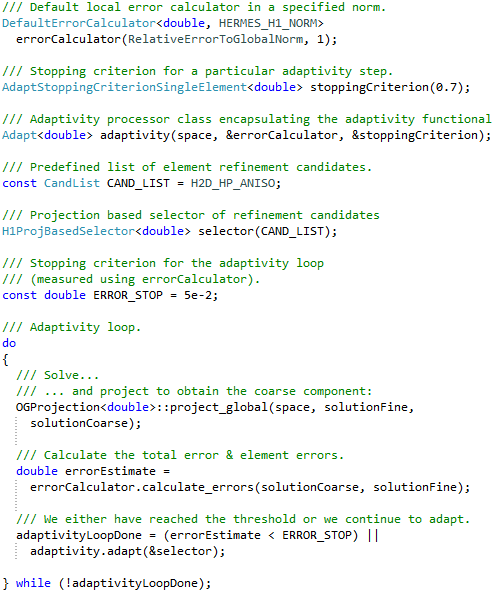
\includegraphics[width=.85\textwidth]{codeimg/adapt.png}
			\caption{Adaptivity API of Hermes}
		\end{subfigure}
		\begin{subfigure}{.49\textwidth}
		\centering
			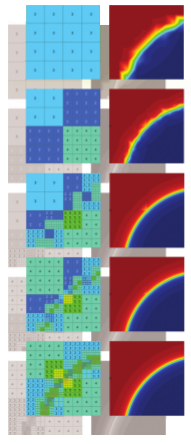
\includegraphics[width=.4\textwidth]{outputs/poster.png}
			\caption{hp-FEM solution of a benchmark}
		\end{subfigure}
	\end{figure}
\end{frame}

\section{Features list}
\begin{frame}
	\begin{itemize}
		\item Unified library for handling both \bbb{real and complex} problems using C++ templating
		\item Library capable of solving problems using \bbb{hp-FEM} and \bbb{hp-DG} methods and their \bbb{combination}
		\item Shared memory parallel code (using \bbb{OpenMP}) tuned for performance
		\item XML \& binary \bbb{export / import} of important algebraic \& FEM-related entities
		\item \bbb{Multimesh}: Calculations with physical quantities defined in different subdomains on separate meshes
		\item Comfortable development: Exception safe API, \bbb{OpenGL} visualization in separate thread
		\item Supported platforms: Linux (Ubuntu, Debian), Windows (MSVC)
		\item Well arranged doxygen \& sphinx \bbb{documentation} with described examples
		\item Generic support (in all physical fields) of \bbb{curved elements}
		\item Shapesets of p-order up to 10 \bb{+} base classes for \bbb{custom shapeset implementations}
	\end{itemize}
\end{frame}

\begin{frame}
\frametitle{hp-FEM examples}
Microwave heating \\
\begin{center}
$$\movie[height=0.5\textheight]{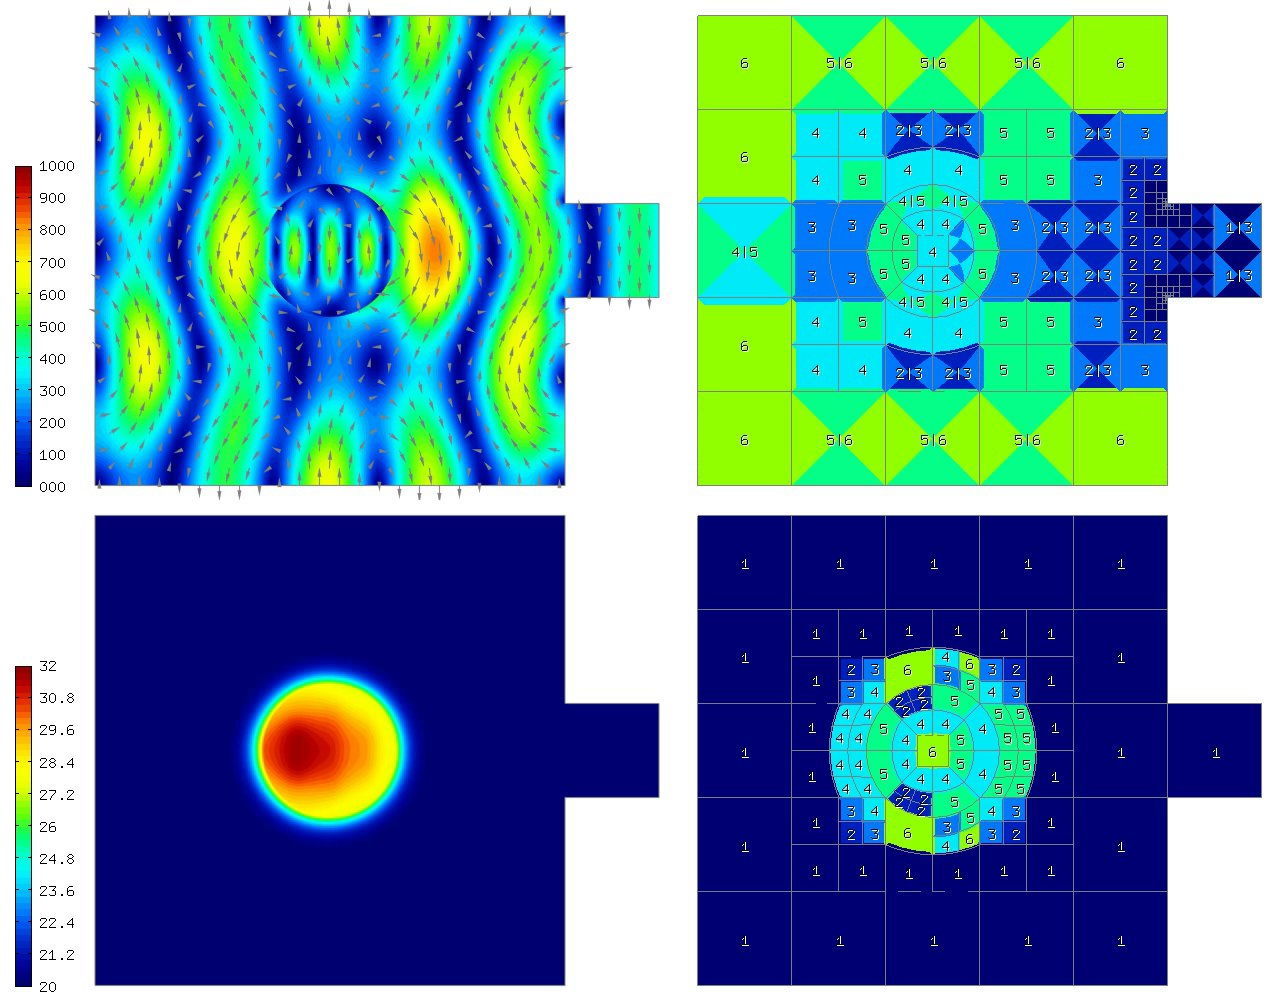
\includegraphics[height=0.5\textheight]{outputs/micro.jpg}}{micro.avi}$$
The microwave model consists of a cavity and a small square waveguide attached to its righ-hand side. The cavity contains a food specimen (load) with temperature-dependent electric permittivity.
\end{center}
\end{frame}

\begin{frame}
\frametitle{hp-FEM examples}
Flame propagation\\
\begin{center}
$$\movie[height=0.52\textheight]{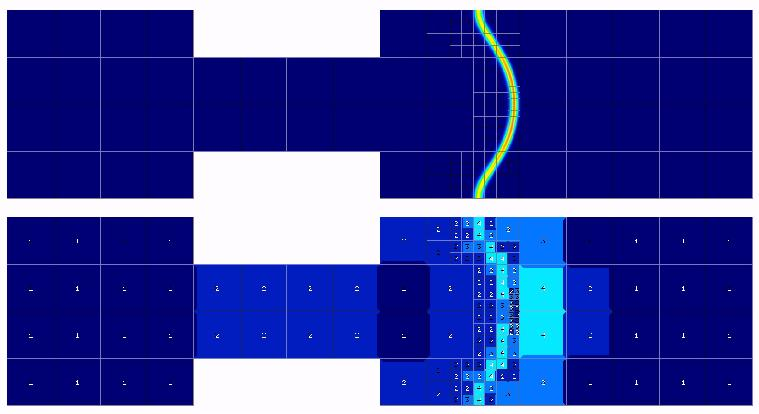
\includegraphics[height=0.52\textheight]{outputs/flame.jpg}}{flame.avi}$$
The underlying model consists of two nonlinear parabolic equations describing the temperature and concentration. The flame moves through the domain from the left to the right.
\end{center}
\end{frame}

\begin{frame}
\frametitle{hp-FEM examples}
Two-component incompressible viscous flow
\begin{center}
$$\movie[height=0.55\textheight]{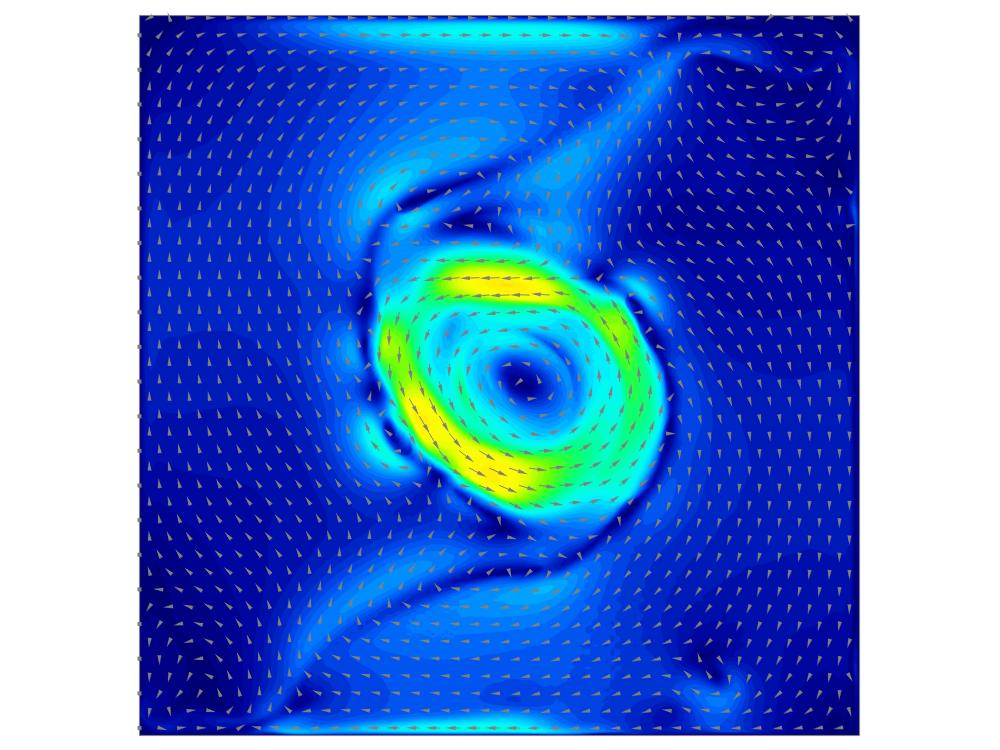
\includegraphics[height=0.55\textheight]{outputs/two_s.jpg}}{velocity.avi}$$
The problem is described by Navier-Stokes equations for two-component flow with some modifications.
\end{center}
\end{frame}


\section{Live presentation}

\begin{frame}
\begin{center}
    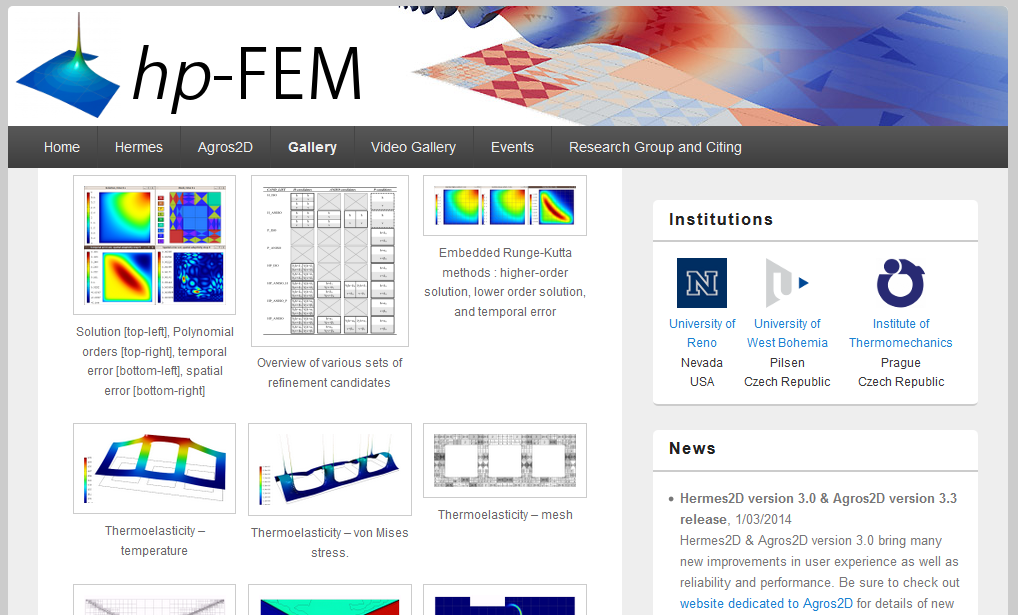
\includegraphics[width=0.8\textwidth]{final.png}\\ \ \\
http://www.hpfem.org/hermes/
\end{center}
\end{frame}
\end{document}
